% \section{Visualization design}
% \subsection{Query execution overview}
% \subsubsection{Execution plan view}
% \subsubsection{Execution progress view}
% \subsection{Task view}
% \subsection{System profiling visualization}
% \subsection{Linkage and interactions}

\section{Visualization design}
Following the data modeling, we present the web-based visual analytics system to support the interactive exploration with four coordinated views. The Execution progress demonstrates the overview about how the query plan are execute(\textbf{T1}), the Task distribution view shows the task distribution and the data dependencies. Integrated with the machine performance metrics, this view is also used for reason the specific patterns of tasks(\textbf{T2} and \textbf{T3}).  Task list provides the detailed information at the task level(\textbf{T2}).  At last, the interaction and linkage are introduced to support the multi-level explorations(\textbf{T4}).

\subsection{Query Progress View}


\begin{figure}[t]
	\centering
	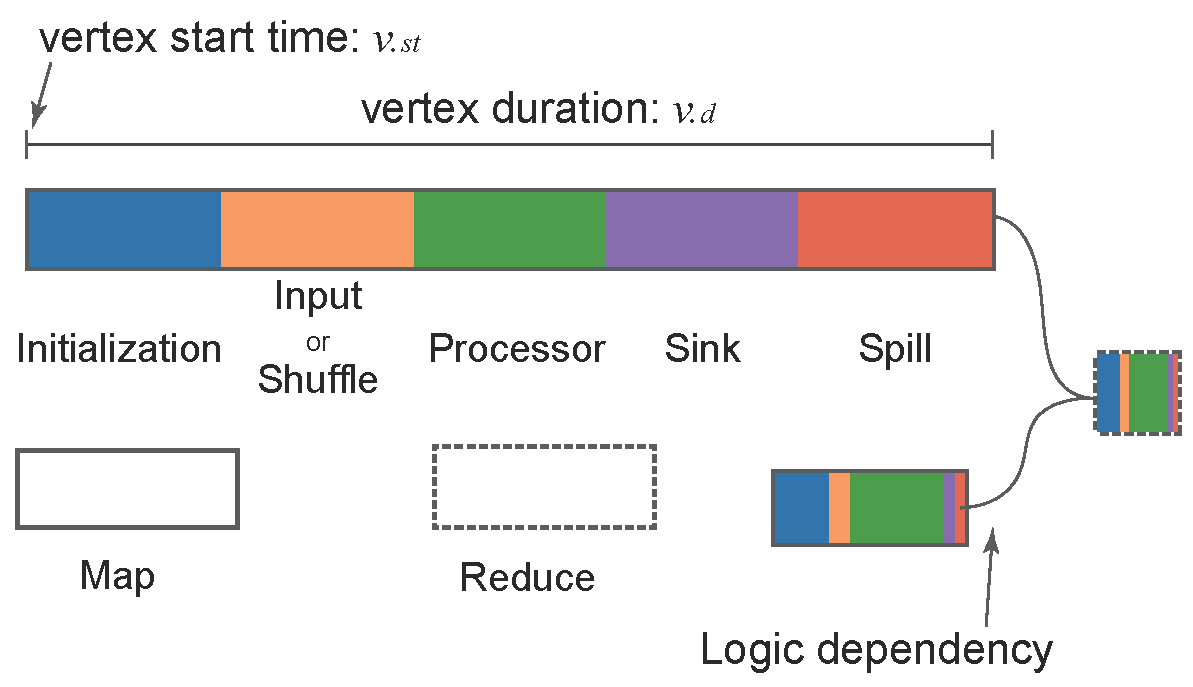
\includegraphics[width=0.40\textwidth]{figures/visualization/progressdesign.pdf}
	\vspace{-3mm}
	\caption{Visual encoding of logic vertex and dependency}
	\label{fig:progress}
	\vspace{-3mm}
\end{figure}


Query Progress View is developed to overview the overall progress of query execution and the logic dependencies. 
The commonly used methods to visualize the progress data is Gantt chart.

As shown by figure~\ref{fig:progress}, the x-axis indicates the timestamp. The rectangles with the same  height indicate the temporal information of logic vertices. Given a vertex $v$, the position of left sides indicates the start time $v.st$ and the duration of $v.d$ is encoded by the length of the rectangle. We use the color to encode the step and the stroke dash style to encode the type of vertex as shown by figure~\ref{fig:progress}.

%\begin{itemize}
%    \item Traditional method: Gantt diagram and design consideration 
%    \item Proposed algorithms, link processing
%    \item Alternative design
%        \begin{itemize}
%            \item Gantt(consider the vertical edge, large space, unclear structure)
%            \item New design loose(clear structure, large space)
%            \item New design compact(small space, unclear structure)
%        \end{itemize}
%\end{itemize}

% -Visual form of Gantt diagram
% -Our design consideration
% -Algorithms
% -Design alternatives
% --gantt(consider the vertical edge, large space, unclear structure)
% --new design loose(clear structure, large space)
% --new design compact(small space, unclear structure)
% --new design compact, edge processing(small space, clear structure)
\subsection{Task view}
\begin{itemize}
    \item Design consideration. Why gantt doesn't work(need very large space, difficult to show the data-flow link, difficult to show and select the abnormal cases)
    \item Our design
    \item Compare with design alternative (Gantt)
\end{itemize}


\subsection{Profiling view}
\begin{itemize}
    \item Our design consideration
    \item Design: Embedding task view to profiling view
    \item Design: Visualize the profiling results
\end{itemize}

\subsection{Interactions}
\begin{itemize}
    \item Multi-scale navigation
    \item Inner and inter linking
\end{itemize}
